%% content.tex
%%

%% ==============================
\chapter{Analytical solution of heat transfer problem}
\label{ch:anaSol}
%% ==============================

The given task is to conduct a one dimensional heat transfer analysis in a rectangular fin with a uniform cross-sectional area A. On one side the fin is fixed to a wall at a given wall temperature $T_{wall} = 300 \deg C$. At the surface of the fin there is convective heat transfer caused by a surrounding fluid with a temperature of $T_{\infty} = 20 \deg C$. The combined heat transfer coefficient between fin surface and fluid is given as $h = 10 \frac{W}{m^{2}K}$. The heat conductivity of the fin material is given to $k = 100 \frac{W}{mK}$.

In the following section the analytical solution for the given heat transfer problem is solved. 
The basic equation is given to $T'' = m^2 (T-T_{\infty})$ according to the assignment.
T can be written as $T = t + T_{\infty}$, which leads to $t = T - T_{\infty}$. 
From this follows $t' = T'$ and $t'' = T''$.
Furthermore $m^{2} = hP/kA_{T}$.
From the equations above, follows a differential equation for t according to $t'' = m^{2}t$.

As a next step to solve the differential equation the eigenvalues and eigenvectors must be calculated. 
\begin{equation}
\begin{cases}
t_{1} = t \\
t_{2} = t'
\end{cases}
						\implies \vec{t'} = 	\begin{pmatrix}	0 & 1\\	m^{2} & 0 \end{pmatrix}  \vec{t}
\end{equation}
The eigenvalues result of the equation $\lambda^{2} = m^{2}$ to $\lambda_{1} = m$ and $\lambda_{2} = -m$.
Therefore the eigenvectors result to $\lambda_{1} = \begin{pmatrix}	1\\	m \end{pmatrix}$ and $\lambda_{2} = \begin{pmatrix}	1 \\	-m \end{pmatrix}$.

This leads to the following equation where the matrix is called the fundamental matrix $Y(x)$ to $\vec{t}(x)$ which is composed of the solution vectors. The solution is therefore a linear combination of the columns of this matrix.
\begin{equation}
\vec{t}(x) = Y(x)\cdot \vec{c} = \begin{pmatrix}	e^{mx} & e^{-mx}\\	me^{mx} & -me^{-mx} \end{pmatrix} \vec{c}
\end{equation}
With $\vec{c} = (C_1 C_2)^T$ it follows that
\begin{equation}
t(x) = e^{mx}C_{1} + e^{-mx}C_{2}.
\label{eq:ODEt}
\end{equation}

To solve this differential equation the following boundary conditions were defined and have to be solved. 

\begin{equation}
\begin{cases}
T(0) = T_w \\
   0 = h(T(L)-T_{\infty})+kT'(L)
\end{cases}
\implies
\begin{cases}
t(0) = T_w-T_{\infty} \\
   0 = ht(L)+kt'(L)
\end{cases}
\end{equation}

Considering the boundary conditions for the left and right edge, two matrices A and B as well as the vector $\vec{r}$ are defined to the following. With $A$ and $B$ reflecting the boundary conditions at $x = 0$ and $x = L$ respectively. $\vec{r}$ gives the source term from the boundary conditions.

\begin{equation}
\label{eq:ABC}
A = \begin{pmatrix}	1 & 0\\	0 & 0 \end{pmatrix}, B = \begin{pmatrix}	0 & 0\\	h & k \end{pmatrix}, \vec{r} = \begin{pmatrix}	T_w-T_{\infty}\\	0 \end{pmatrix} = \begin{pmatrix}	\Delta T \\	0 \end{pmatrix}
\end{equation}

With the identities from \autoref{eq:ABC}, R is given as
\begin{equation}
R = \begin{pmatrix}	1 & 1\\	\underbrace{he^{mL}+mke^{mL}}_{a} & \underbrace{he^{-mL}-mke^{-mL}}_{b} \end{pmatrix} = A \cdot Y(0)+B \cdot Y(L)
\end{equation}

To calculate the constants $C_1$ and $C_2$ for the differential \autoref{eq:ODEt} the following system given by $R \vec{c} = \vec{r}$ of equations must be solved.

\begin{equation}
\begin{aligned}
	&\left(\begin{array}{cc|c}
		1 & 1 & \Delta T \\
		a & b & 0 \\
	\end{array} \right)
	\xrightarrow[]{l_2 - \frac{l_2}{b}}
	\left(\begin{array}{cc|c}
		1-\frac{a}{b} & 0 & \Delta T \\
		a & b & 0  \\
	\end{array}\right)\\
	\xrightarrow[l_2-\frac{l_1}{a-\frac{a}{b}}]{}&
	\left(\begin{array}{cc|c}
		1 & 0 & \frac{\Delta T}{1- \frac{a}{b}}\\
		0 & b & \frac{-\Delta T \cdot a}{1-\frac{a}{b}}\\
	\end{array}\right)
	\rightarrow
	\left(\begin{array}{cc|c}
		1 & 0 & \frac{\Delta T}{1-\frac{a}{b}}\\
		0 & 1 & \frac{-\Delta T}{1-\frac{a}{b}} \cdot \frac{a}{b}\\
	\end{array}\right)
\end{aligned}
\end{equation}

\begin{equation}
C_1 = \frac{\Delta T}{1 - \frac{a}{b}}
\end{equation}

\begin{equation}
C_2 = \frac{-\Delta T}{1 - \frac{a}{b}} \cdot \frac{a}{b}
\end{equation}

Using the values of $C_1$ and $C_2$ in \autoref{eq:ODEt} the solved differential equation for t results in
\begin{equation}
\label{eq:tfinal}
t(x) = e^{mx} \cdot \frac{\Delta T}{1 - \frac{a}{b}} + e^{-mx} \cdot \frac{-\Delta T}{1 - \frac{a}{b}} \cdot \frac{a}{b}.
\end{equation}

Therefore the solution of $T(x)$ follows form \autoref{eq:tfinal} and $T(x) = t + T_{\infty}$ as 

\begin{equation}
T(x) = e^{mx} \cdot \frac{\Delta T}{1 - \frac{a}{b}} - e^{-mx} \cdot \frac{\Delta T}{1 - \frac{a}{b}} \cdot \frac{a}{b} + T_\infty.
\end{equation}


\chapter{Matlab code for heat transfer problem}
\label{ch:matlabcode}

In the upcoming chapter the matlab code programmed for the heat transfer problem will be presented and discussed. 

%XXX
%Soll der Anfang der auskommentiert ist auch erklärt werden? Der wird doch gar nicht verwendet oder? Soll der dann überhaupt im Code sein?
%XXX

The following \autoref{fig:defineconstants} shows the beginning of the matlab code used for the heat transfer problem. 

\begin{figure}[H]
    \centering
    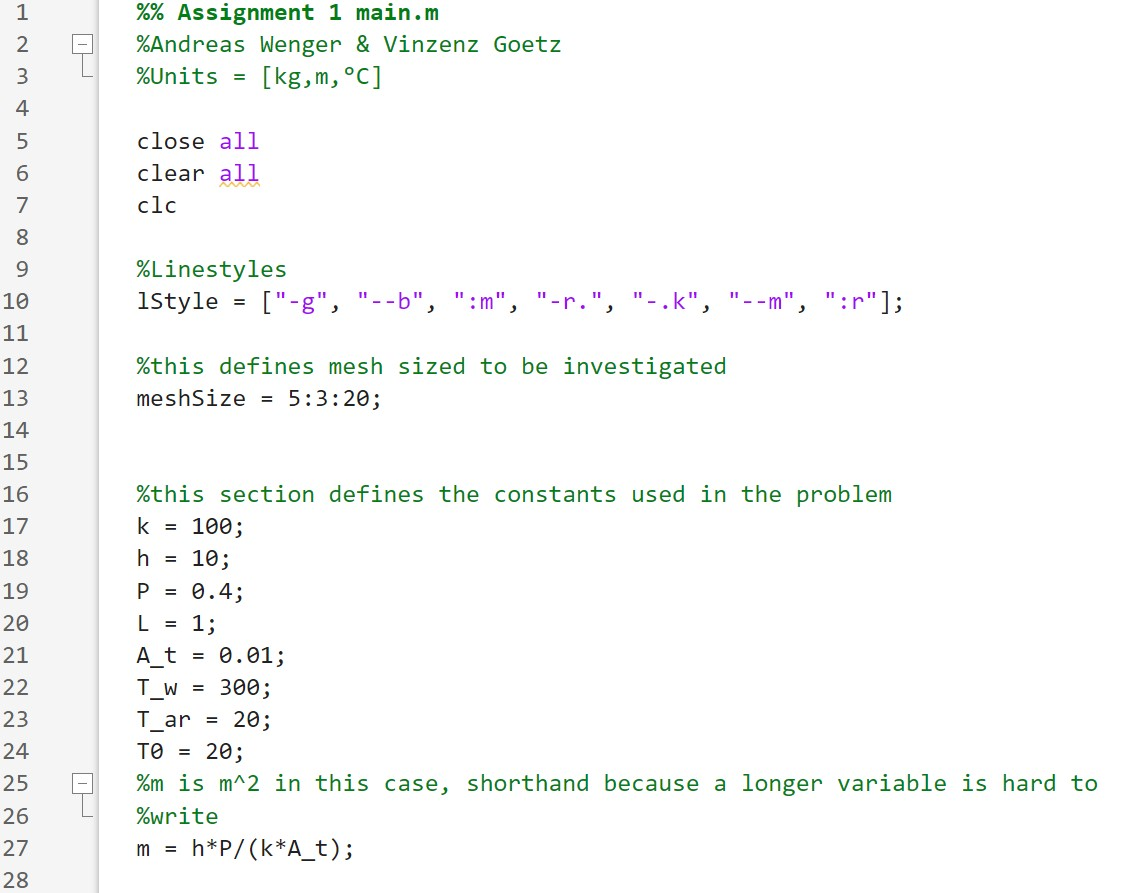
\includegraphics[width=.8\textwidth]{figures/define_constants.jpg}
    \caption{The matlab code for the definition of the constants used in this problem}
    \label{fig:defineconstants}
\end{figure}

At first all existing windows are closed, the storage of variables is erased and the command window is cleared. 
%After that the linestyles for the figures using multiple input variables are stated. 
The mesh size is choosen to vary from 5 to 20 elements using a step size of 3. In total 6 different mesh sizes are compared in this study. As described later the relative error using more than 20 mesh elements will not drop siginicantly. Therefore the maximum mesh size is limited to 20 in order to save computing time. 

The next section of the code defines the constants used in the problem as given in the assignment. For convenience of the reader and writer the variable used for $m^2$ is $m$.  

As the analytical solution is already obtained in \autoref{ch:anaSol}, the subsequent \autoref{fig:defineconstantsanaSol} depicts a further constant being defined, which is given as $\gamma = \frac{\Delta T}{1-\frac{a}{b}}$. Furthermore the error vector is initialized with the right length. 


\begin{figure}[H]
    \centering
    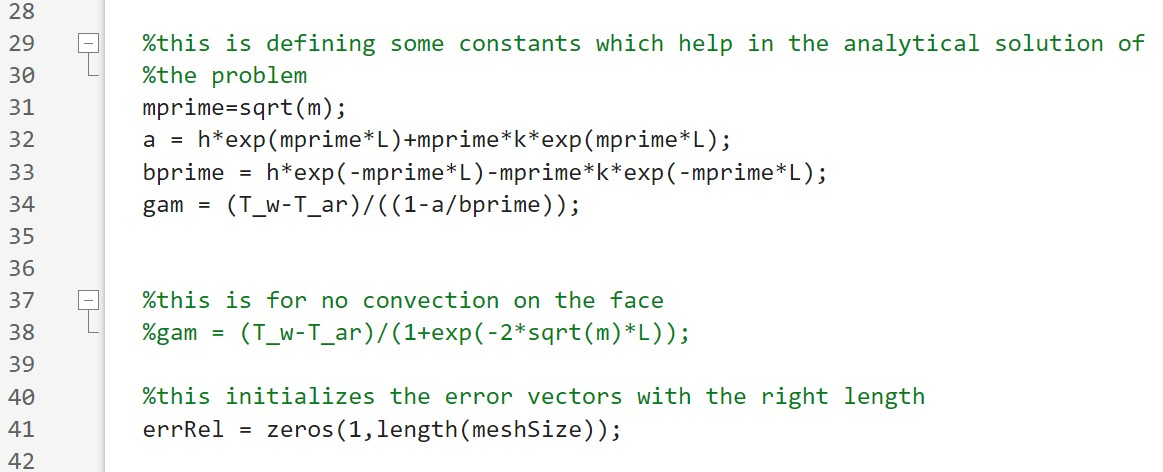
\includegraphics[width=.8\textwidth]{figures/define_anaSol_constants.jpg}
    \caption{The matlab code for the definition of further constants using the analytical solution}
    \label{fig:defineconstantsanaSol}
\end{figure}



The following fragment of our matlab code initializes a for loop to calculate the given heat transfer problem for multiple mesh elements sequentially. This is shown in \autoref{fig:calculateT}.


\begin{figure}[H]
    \centering
    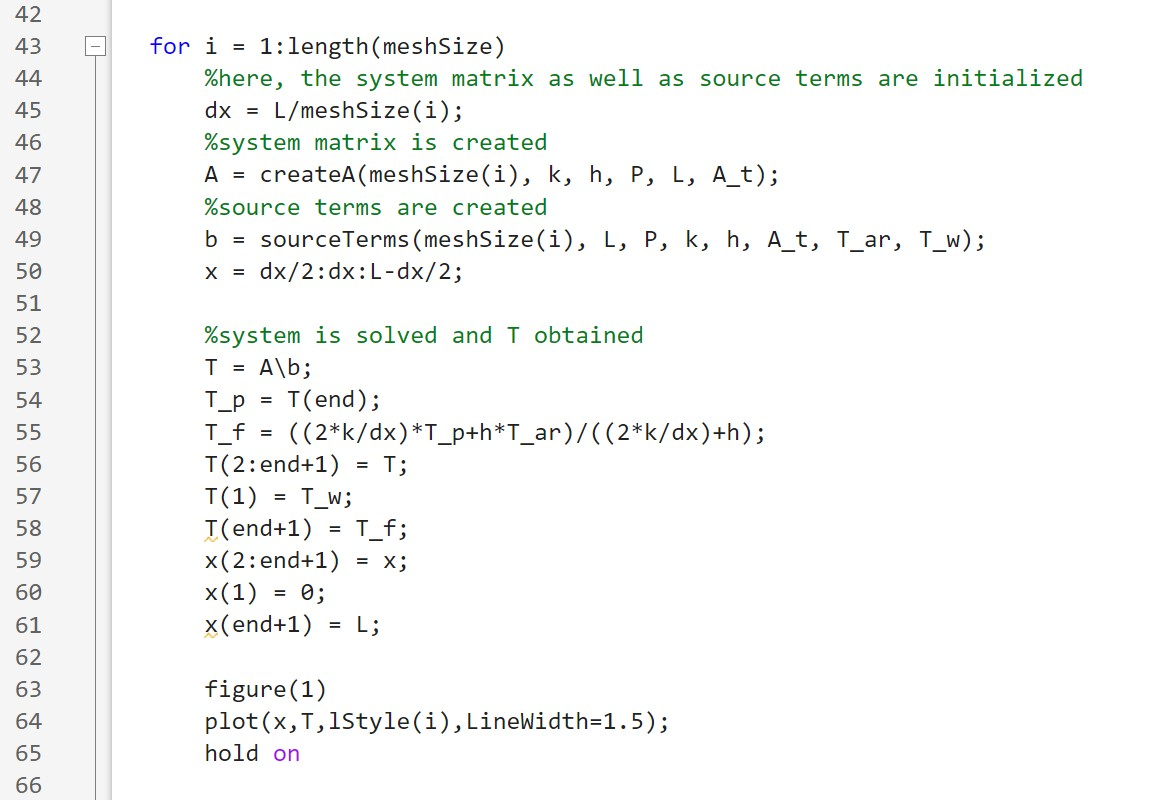
\includegraphics[width=.8\textwidth]{figures/begin_for_loop_calculate_T.jpg}
    \caption{The matlab code for the calculation of T}
    \label{fig:calculateT}
\end{figure}

For the calculation to work properly, at first $dx$ is defined. Afterwards the system matrix as well as the source terms are initialized with the functions A = createA() and b = sourceTerms().

createA takes as arguments the mesh elements, k, h, P, L, and the area of the fin tip. Where k is the heat conductiveness, h the heat transfer coefficient, P the perimiter of the fin and L the length. It returns the sparse system matrix for the heat conduction problem, which was defined in the assignment.

sourceTerms takes the mesh elements, L, P, k, h, the area of the tip, the temperature of the surrounding fluid and the temperature of the wall. L, p, k and h are defined as in createA. This function returns a vector of source terms also defined in the assignment.


The next step is calculating the numerical solution for $T$ at the cell midpoints. This is done by the built-in function of Matlab to solve a system of linear equations which solves $A\vec{x} = b$ by x = A\textbackslash b. Moreover the temperature $T_f$ at the end of the rod is calculated and the vector T shifted and the first entry set to $T_{wall}$. Also, the vector $x$ of cell centroid positions is shifted by 1 to account for the face of the cell of the wall and also lengthened by 1 to account for the face of the tip.


The temperature $T$ is then plotted into figure(1) as seen in \autoref{fig:calculateT}. 

Upcoming \autoref{fig:calcanaSol} shows matlab code for calculating the analytical solution as well as displaying the relative errors. 

\begin{figure}[H]
    \centering
    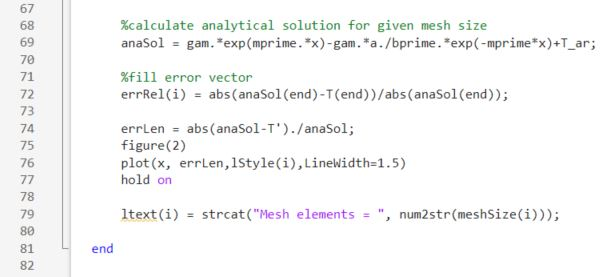
\includegraphics[width=.7\textwidth]{figures/calculate_anaSol_fill_errvec.jpg}
    \caption{The matlab code for the calculation of the analytical solution and the display of relative errors}
    \label{fig:calcanaSol}
\end{figure}

The error vectors shown in figure \autoref{fig:errLen} display the relative error between the numerical solution and the analytical solution over the length of the rod at different numbers of mesh elements. 

The relative error at the last point of the rod is displayed in figure \autoref{fig:errElems}. As shown, the relative error decreases with increasing numbers of mesh elements. 

\begin{minipage}[H]{.45\textwidth}
\begin{figure}[H]
    \centering
    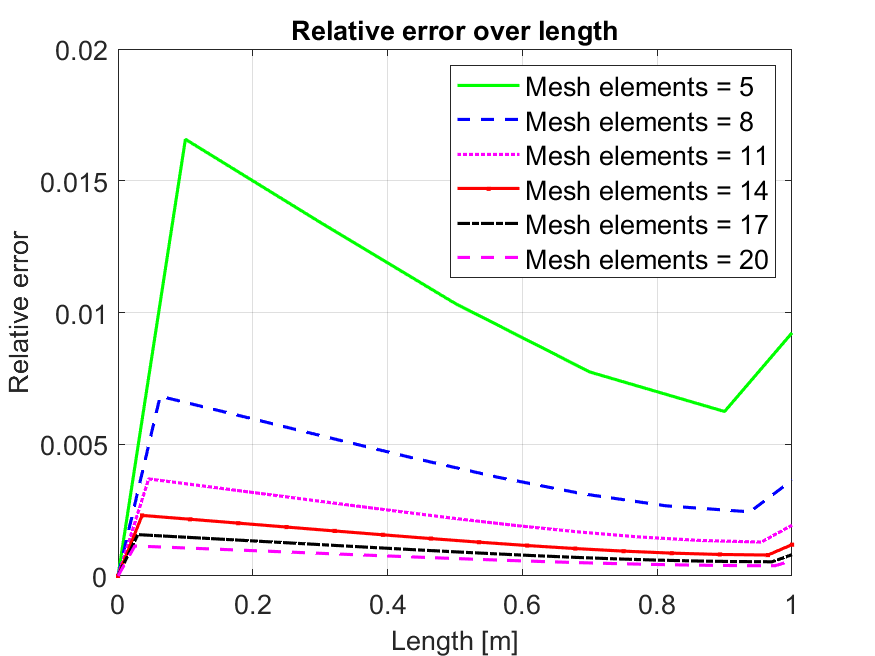
\includegraphics[width=\textwidth]{figures/errLen.png}
    \caption{The relative error of $T$ over the length of the rod with a varying number of mesh elements.}
    \label{fig:errLen}
\end{figure}
\end{minipage}
\begin{minipage}[H]{.45\textwidth}
\begin{figure}[H]
    \centering
    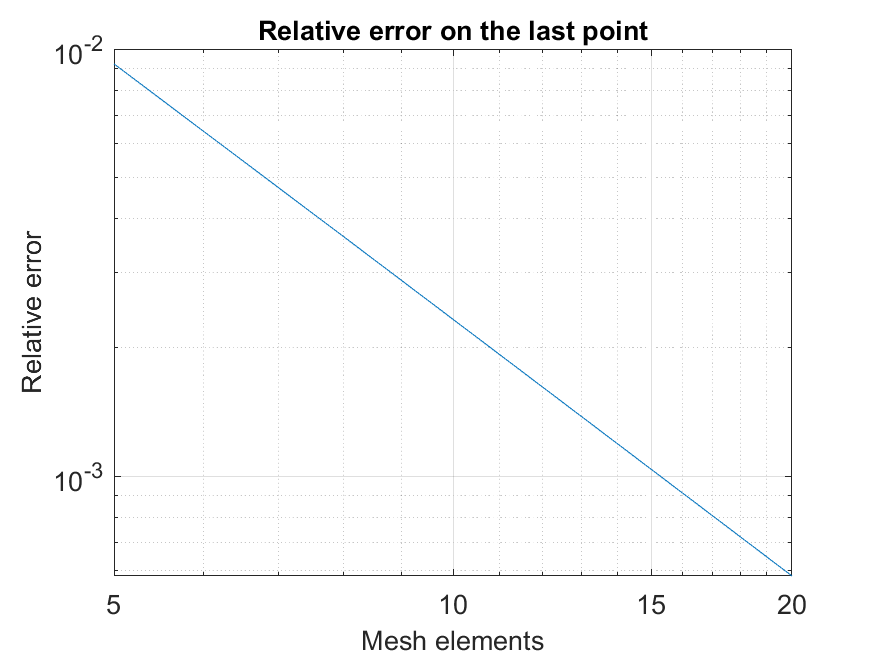
\includegraphics[width=\textwidth]{figures/errElems.png}
    \caption{The matlab code for the relative error at the last point comparing different numbers of mesh elements.}
    \label{fig:errElems}
\end{figure}
\end{minipage}


\begin{figure}[H]
    \centering
    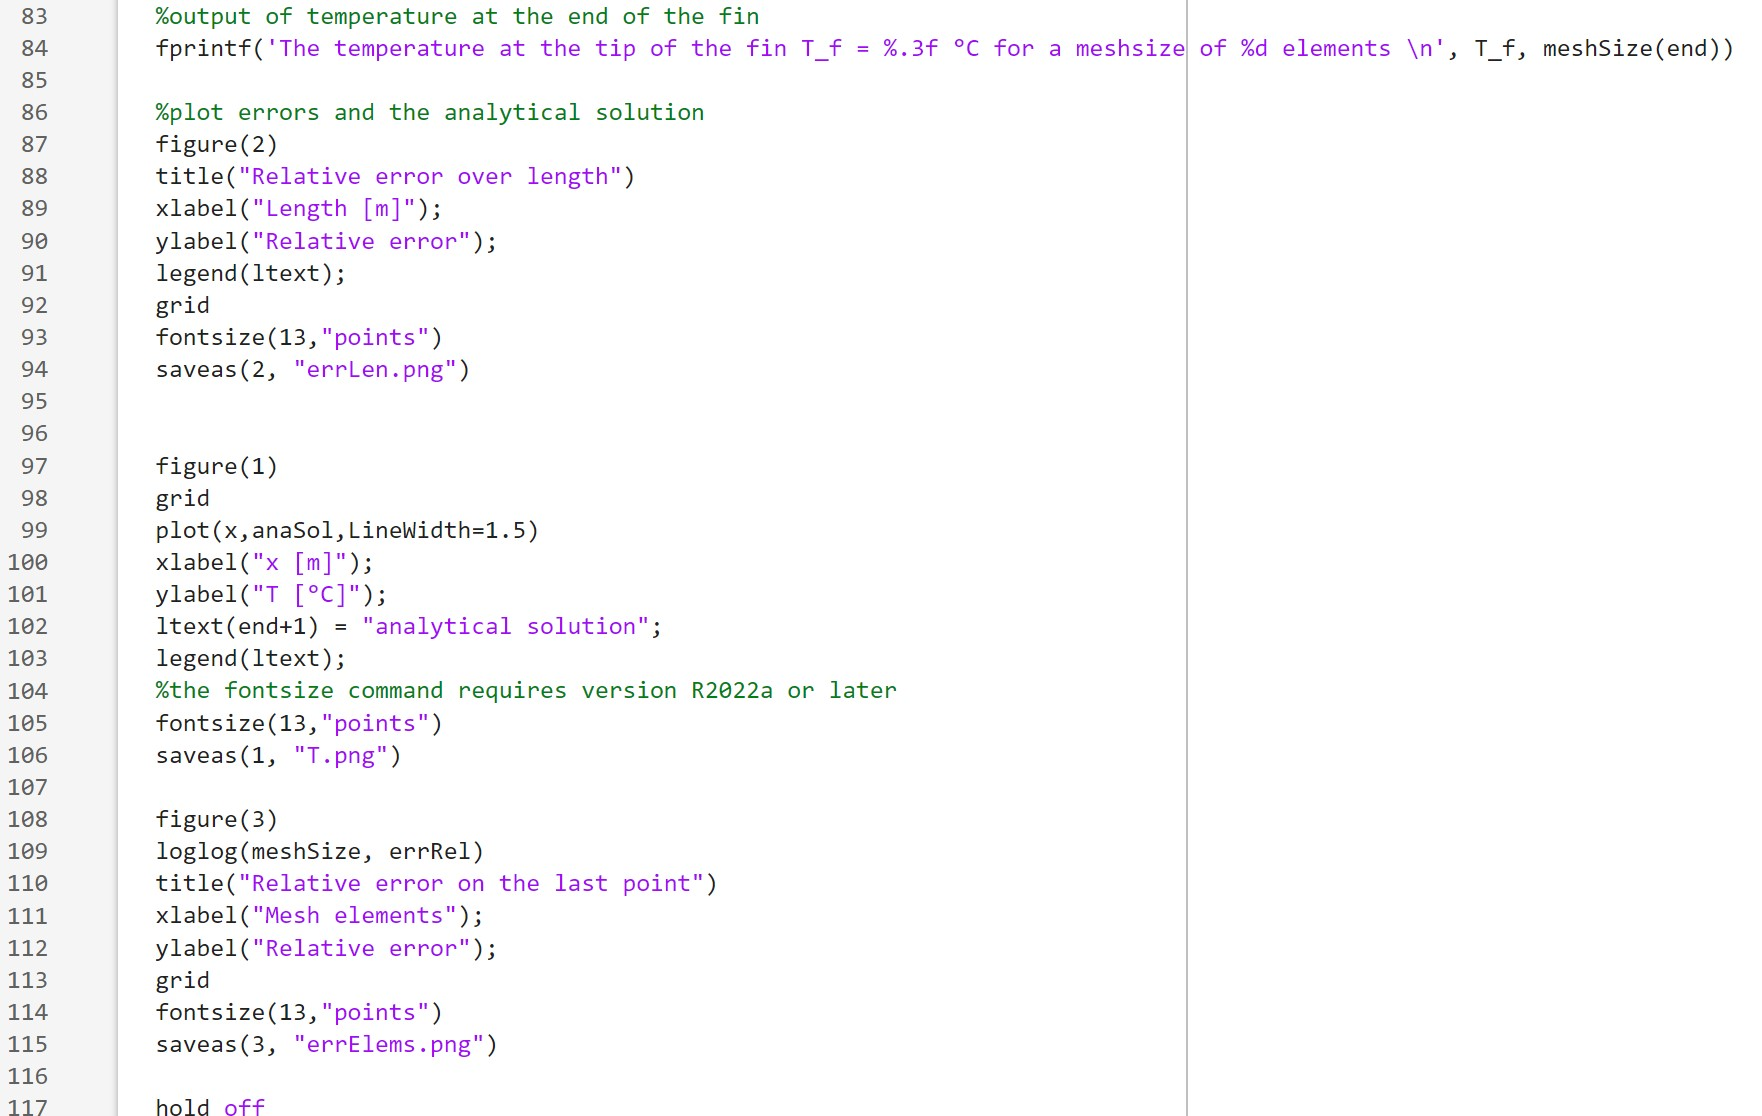
\includegraphics[width=.8\textwidth]{figures/output_figures.jpg}
    \caption{The matlab code for the output $T_f$ and temperature curves of different numbers of mesh elements compared to the analytical solution.}
    \label{fig:output}
\end{figure}

\autoref{fig:output} depicts the matlab code used for the output. 


The temperature at the tip of the fin $T_f$ is posted into the command window of matlab for the biggest number of mesh elements investigated.

Furthermore the temperature curve for the analytical solution is displayed in \autoref{fig:T}. It can be seen that the difference between variing numbers of mesh elements and the analytical solution is small. 

\begin{figure}[H]
    \centering
    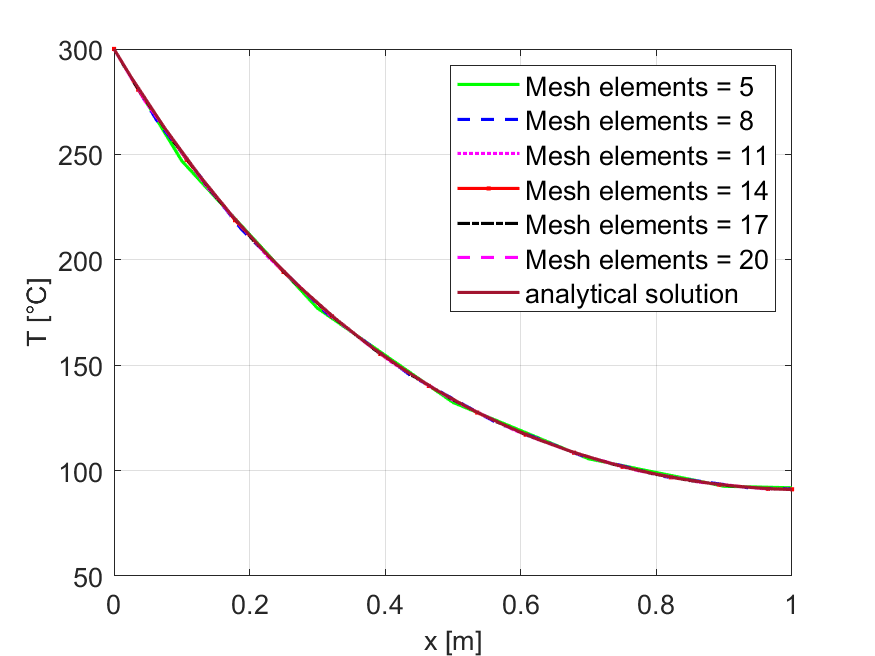
\includegraphics[width=.75\textwidth]{figures/T.png}
    \caption{The matlab code for the output temperature curves of different numbers of mesh elements compared to the analytical solution.}
    \label{fig:T}
\end{figure}


















